% Experiments Section - Concise NeurIPS style

We evaluate \ours{} on three benchmarks: FB15k-237 (237 relations), YAGO3-10 (37 relations), and WN18RR (11 relations).
We compare against DistMult~\citep{yang2015embedding} and GGPN~\citep{chen2022graph}, using identical DistMult scoring and BCE loss for fair comparison.
We measure link prediction (MRR, Hits@10), OOD detection (AUROC), and calibration (ECE).
Implementation details are in Appendix~\ref{app:implementation}.

\subsection{Main Results}

\begin{table}[t]
\centering
\caption{Results on FB15k-237 (mean $\pm$ std, 3 seeds). \ours{} achieves \textbf{55\% higher AUROC} than DistMult.}
\label{tab:main}
\vspace{0.5em}
\begin{tabular}{lcccc}
\toprule
Model & MRR $\uparrow$ & Hits@10 $\uparrow$ & ECE $\downarrow$ & AUROC $\uparrow$ \\
\midrule
DistMult & \textbf{0.264} & \textbf{0.433} & \underline{0.082} & 0.550 \\
GGPN & 0.249 & 0.416 & \textbf{0.079} & 0.221 \\
\ours{} & \underline{0.255} & \underline{0.413} & 0.118 & \textbf{0.854} \\
\bottomrule
\end{tabular}
\end{table}

Table~\ref{tab:main} shows our main results on FB15k-237.
\ours{} achieves AUROC of \textbf{0.854}, compared to 0.550 for DistMult (+55\%) and 0.221 for GGPN.
Notably, GGPN's AUROC below 0.5 indicates \emph{inverted} uncertainty---it assigns higher uncertainty to in-distribution samples.
\ours{} maintains competitive link prediction (MRR 0.255 vs 0.264).

On YAGO3-10 (37 relations), \ours{} achieves AUROC 0.830 vs DistMult's 0.619 (+34\%), confirming the benefit of relation-aware kernels on relation-rich KGs.

\subsection{When Does \ours{} Work?}

\begin{table}[t]
\centering
\caption{OOD detection across datasets. \ours{} excels when \#relations $\geq 30$.}
\label{tab:threshold}
\vspace{0.5em}
\begin{tabular}{lcccl}
\toprule
Dataset & Relations & \ours{} & DistMult & $\Delta$ \\
\midrule
WN18RR & 11 & 0.629 & \textbf{0.860} & $-27\%$ \\
YAGO3-10 & 37 & \textbf{0.830} & 0.619 & $+34\%$ \\
FB15k-237 & 237 & \textbf{0.854} & 0.550 & $+55\%$ \\
\bottomrule
\end{tabular}
\end{table}

Table~\ref{tab:threshold} and Figure~\ref{fig:threshold} reveal a critical finding: \ours{}'s effectiveness depends on \textbf{relation density}.
On WN18RR (11 relations), per-relation kernels provide insufficient differentiation.
The threshold is approximately \textbf{30 relations}---above this, \ours{} consistently outperforms baselines.

\begin{figure}[t]
\centering
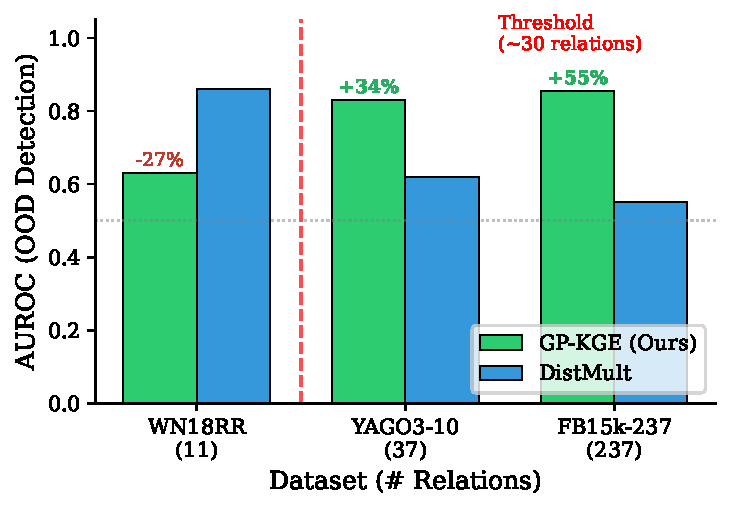
\includegraphics[width=0.8\linewidth]{figures/relation_threshold.pdf}
\caption{OOD detection performance vs relation density. GP-KGE excels when \#relations $\geq 30$.}
\label{fig:threshold}
\end{figure}

\subsection{Ablations}

\paragraph{Graph Initialization.}
Initializing embeddings from graph Laplacian eigenvectors improves ECE by \textbf{44\%} (0.099$\to$0.055) while maintaining AUROC.

\paragraph{Global Kernel.}
On WN18RR, adding a global kernel (ignoring relation types) improves ECE by \textbf{64\%} (0.144$\to$0.051), providing a fallback for relation-sparse KGs.
